\documentclass[size=A4]{scrreprt}

\usepackage[utf8x]{inputenc}
\usepackage[ngerman]{babel}
\usepackage{listings}
\usepackage{caption}
\usepackage{graphicx}
\usepackage{color}
\usepackage{todonotes}
\usepackage{mathtools}
\usepackage{float}
\usepackage{sidecap}

\sidecaptionvpos{figure}{t}
\definecolor{mygreen}{rgb}{0.08,0.35,0}
\definecolor{mygray}{rgb}{0.9,0.9,0.9}
\definecolor{mymauve}{rgb}{0.58,0,0.82}

\DeclareCaptionFormat{listing}{
  \colorbox[rgb]{1.0, 1.0, 1.0 }{
    \parbox{\textwidth}{\hspace{17pt}#1#2#3}
  }
}
\captionsetup[lstlisting]{ format=listing,  singlelinecheck=false, margin=0pt, font={bf,footnotesize} }

\title{Ein Vergleich der Verifikationswerkzeuge Verifast und Frama-C}
\author{Georg Wächter\\Humboldt Universität zu Berlin}
\date{Februar 2014}

\lstset{
  backgroundcolor=\color{white}, 
  basicstyle=\ttfamily\small,     
  breakatwhitespace=false,      
  breaklines=true,                
  captionpos=b,                  
  commentstyle=\color{mygreen},    
  extendedchars=true,       
  frame=single,                 
  keywordstyle=\color{blue},     
  language=Octave,               
  morekeywords={bool},       
  numbers=left,               
  numbersep=5pt,                
  numberstyle=\color{black},
  rulecolor=\color{black},  
  stepnumber=1,       
  stringstyle=\color{mymauve},  
  tabsize=2,   
  columns=fixed,                  
}

\usepackage{geometry}
\geometry{a4paper,left=30mm,right=30mm, top=2cm, bottom=2cm} 

\begin{document}

\maketitle
\tableofcontents

\chapter{Einleitung}

\section{Aufgabenstellung und Durchführung}
\label{sec:aufgabenstellung}
Diese Arbeit vergleicht die statischen Verifikationswerkzeuge Verifast\footnote{
\url{http://people.cs.kuleuven.be/~bart.jacobs/verifast/}} und ACSL\footnote{\url{http://frama-c.com/acsl.html}} 
in Kombination mit Frama-C\footnote{\url{http://frama-c.com}}. 
Der Fokus liegt dabei auf einfachen Algorithmen, die mit Arrays arbeiten ohne sie zu verändern.
Dabei wird die Lesbarkeit, Ausdrucksstärke sowie der notwendige manuelle Aufwand der Verifikation betrachtet.
Für den praktischen Einsatz wichtige Faktoren werden ebenso untersucht. Das sind insbesondere die verfügbare 
Dokumentation, die Integration in den Entwicklungsprozess und die Geschwindigkeit der Werkzeuge.
\newline
\newline
Als durchgängiges Beispiel dient in dieser Arbeit der standardisierte mismatch-Algorithmus\footnote{siehe
\url{http://msdn.microsoft.com/de-de/library/f0bsxbk9.aspx}} aus
der C++ Standard-Bibliothek. Die Grundlage für spätere Formalisierung ist die folgende vereinfachte\footnote{es
wird auf Iteratoren und eine selbst definierte Vergleichsfunktion verzichtet} Signatur und 
die dazugehörige informelle Spezifikation:

\lstset{frame=none, numbers=none}    
\lstinputlisting[language=C]{codes/mismatch_signature.c}
\lstset{frame=single, numbers=left}

\noindent \emph{Vergleicht die Elemente der beiden Arrays beginnend bei 0 bis einschließlich size - 1 und gibt den
Index der ersten Elemente zurück, die sich unterscheiden. Sind alle Elemente gleich, gibt der Algorithmus
size - die Länge der Liste - zurück.}
\newline
\newline
Auf Grund des einfachen Beispiels hat der Vergleich nur eine begrenzte Aussagekraft, denn es werden nicht alle
Spracheigenschaften von Verifast bzw. ACSL gezeigt und verglichen. Zudem kommt hinzu, dass sich beide Werkzeuge
kontinuierlich - in ihre jeweils eigene Richtung - weiterentwickeln. Es wird darum immer Anwendungsfälle geben,
in denen ein Werkzeug dem anderen überlegen ist oder sogar alternativlos ist.


\section{Verifast}
\label{sec:verifast}



KU Löwen university, by bart jacobs


for C and java


functional correctness


seperation logic - angepasste hoare logic


malloc/free - keien speicherlöscher


multithreading .. z.B. lock free datenstrukturen

kein eigener name für die sprache, darum wird immer nur von verifast gesprochen


industrieeinsatz

\section{Frama-C}
\label{acsl-und-frama-c}

ansi/iso-c specification language


zusammen mit verifast teil des STANCE projekts

\section{Zielgruppe}
\label{sec:zielgruppe}

Für das Verstehen der Arbeit sollte der Leser die Grundlagen der Programmiersprache C beherrschen.
sowie theoretische Kenntnisse zur Aussagen- und Prädikatenlogik besitzen.
Konkrete Erfahrungen mit ACSL und Frama-C sind hilfreich, da beim Vergleich der Werkzeuge an vielen
Stellen Verifast detaillierter als ACSL erläutert wird. Die Arbeit ist darum auch als Einstieg in Verifast
für ACSL-Nutzer geeignet und ausgelegt.

 



\chapter{Theoretische Grundlagen}

In diesem Kapitel werden die theoretischen Grundlagen der beiden Verifikationswerkzeuge kurz erläutert. Dabei wird bewusst
auf ausführliche Formalismen verzichtet, diese können in den Quellen bei Bedarf nachgelesen werden.

Als erstes wird der Hoare-Kalkül beschrieben - die Grundlage der Softwareverifikation von Frama-C als auch VeriFast.
Anschließend werden die Begriffe der partiellen und totalen Korrekheit im Zusammenhang mit der Terminierung eines Programms
eingeführt. Der letzte Abschnitt widmet sich der Separierungslogik - der theoretischen Basis für die Verifizierung
mit VeriFast.

\section{Hoare-Kalkül}

Der Hoare-Kalkül ist ein formales System zum Beweisen der Korrektheit von Programmen. Es verwendet eine Reihe logischer
Regeln und Axiome, die direkt auf den Quellcode angewendet werden und mit sogenannten Hoare-Tripeln arbeiten. Ein solches
Tripel beschreibt den Zustand vor und nach der Ausführung eines Programmteils mit Hilfe von prädikatenlogischen
Formeln.
\begin{displaymath}
\{P\} \: S \: \{Q\}
\end{displaymath}
Die Formel P gilt vor, Q hingegen nach der Ausführung von S. Damit kann nun die Ableitungsregel zur Komposition von
zwei aufeinander folgenden Programmabschnitten aufgestellt werden:
\begin{displaymath}
\frac{\{P\} \:S\: \{R\} \:, \: \{R\} \: T \: \{Q\}}{\{P\}\: S; T \: \{Q\}}
\end{displaymath}
Die Regeln besagen, dass die unter dem Strich stehende Aussage aus der über dem Strich notierten Aussage folgt. In diesem
Fall beschreibt die Regel die Verkettung zweier Tripel.

Da die im Fokus stehenden Algorithmen mit Schleifen arbeiten, sei hier noch die Iterationsregel gezeigt, die auf While-Schleifen
bzw. auf For-Schleifen im C-Code angewendet wird: 
\begin{displaymath}
\frac{\{I \land B\} \:S\: \{I\}}{\{I\}\: while(B)\: S\: \{I \land \neg B\}}
\end{displaymath}
I bezeichnet die Schleifeninvariante, S den Schleifenkörper und B die Eintrittsbedingung. Kann nachgewiesen werden,
dass S die Invariante erhält und vor der Ausführung B und~I wahr sind, dann gilt die unter dem Strich stehende Aussage: Nachdem
die Schleife durchlaufen ist, gilt nicht B und weiterhin die Invariante. B und S sind direkt aus dem Quellcode entnommen, 
die Schleifeninvariante hingegen muss bei der Verifizierung  manuell angegeben werden (siehe dazu den Abschnitt über 
Schleifeninvarianten im Kapitel 4).

Für die Verifizierung müssen nun alle Regeln auf den Quellcode angewendet werden. Eine von Frama-C verwendete Variation des Hoare-Kalküls
stellt das System der schwächsten Vorbedingungen (engl. weakest preconditions) dar. Dabei findet eine Rückwärtsanalyse
des Quellcodes statt. Begonnen wird mit den zu beweisenden Nachbedingungen. In jedem Schritt wird dann die schwächste Vorbedingung
abgeleitet, sodass am Ende zu beweisen ist, dass die zuletzt berechnete Vorbedingung aus der Vorbedingung des Kontrakts folgt.
Ist dieses Vorgehen erfolgreich, so erfüllt der Quellcode die gegebene Spezifikation aus Vor- und Nachbedingung.

\section{Terminierung}

Mit Hilfe des Hoare-Kalküls lässt sich nicht nachweisen, dass ein Programm terminiert, d.h. nach endlich vielen Schritten 
beendet ist. Man spricht deshalb von der partiellen Korrektheit, da das Programm nur dann das gewünschte 
Verhalten zeigt, wenn es auch tatsächlich zum Ende kommt.

Die Iterationsregel lässt sich z.B. auch dann anwenden, wenn es sich um eine Endlosschleife handelt. Der Nachweis,
dass die Schleife tatsächlich terminiert, ist zusätzlich zu erbringen. 

Die folgende erweiterte Iterationsregel erbringt bei Anwendung genau diesen Beweis. Für die entsprechende Schleife ist damit, die
sogenannte totale Korrektheit gezeigt:
\begin{displaymath}
\frac{\{I \land B \land t = z \} \:S\: \{I \land t < z\}, I \implies t \geq 0}{\{I\}\: while(B)\: S\: \{I \land \neg B\}}
\end{displaymath}

Diese erweiterte Regel ergänzt die als \lstinline{t} bezeichnete Schleifenvariante. Durch die zusätzliche Bedingung, dass aus der gültigen Invariante
eine positive Variante folgt, ergibt sich die Terminierung der Schleife. Denn in jedem Schleifendurchlauf verringert sich die Variante,
sodass letztendlich irgendwann ein Ende erreicht sein muss\footnote{Die Variante t könnte in diesem Fall mit natürlichen Zahlen arbeiten,
das Prinzip ist aber nicht darauf beschränkt, siehe dazu die formalen Ausführungen in \cite{floyd}[Seite 31].}.

Der Nachweis der totalen Korrektheit wird in dieser Arbeit für die vorgestellten einfachen Algorithmen angestrebt.
Allerdings ist es nicht möglich die Terminierung für beliebige Algorithmen zu beweisen, da es sich um ein nicht entscheidbares 
Problem handelt\footnote{Der Mathematiker Alan Turing hat bereits 1936 bewiesen, dass es keinen Algorithmus gibt, der 
entscheiden kann, dass ein beliebiger Algorithmus zum Ende kommt\cite{turing}[Seite 230-265].}.

\section{Separierungslogik}
\label{sec:theorie:seperation-logic}

Die Separierungslogik ist eine Erweiterung des Hoare-Kalküls, die weitergehende Aussagen über den Speicherinhalt
und den Zugriff darauf erlaubt. Die Bedeutung des Hoare-Tripels wird dazu etwas erweitert -- der Programmcode des
betrachteten Tripels darf nur noch auf den Speicher zugreifen, der in der Vorbedingung erwähnt oder aber im Code
allokiert wurde\cite{reynolds-2002}[Kapitel 4].

Außerdem wird die von Hoare definierte zugrunde liegende Programmiersprache erweitert, um Befehle zum Anfordern (engl. allocate), 
Löschen, Manipulieren und Auslesen des Speichers. Der Ausführungszustand wird um zwei neue Komponenten erweitert, damit 
diese Aktionen abgebildet werden können: Der dynamische Speicherbereich (engl. heap) verknüpft Adressen mit ihren
Werten; die lokalen Variablen (engl. store/stack) assoziieren die Namen der Variablen mit ihren Inhalten. 

Die neu eingeführten Konstrukte sind bewusst stark angelehnt an die maschinennahen Konzepte der Zeigerarithmetik sowie des
Stapelspeichers. Somit ist die Anwendung der Logik auf C-Programme leicht möglich.

Damit Vor- und Nachbedingungen Aussagen über den Speicher treffen können, erweitert die Separierungslogik die
von Hoare verwendete Prädikatenlogik um folgende Operatoren bzw. Atome: 
\begin{align*}
\langle Aussage \rangle & ::= \dots \\
& \begin{array}{l r}
  | \: \textbf{emp} & \textrm{leerer Speicher}\\
  | \: \langle Ausdruck \rangle \to \langle Ausdruck \rangle & \textrm{einzelner Wert im Speicher}\\
  | \: \langle Aussage \rangle \ast \langle Aussage \rangle & \textrm{disjunkte Speicherbereiche, Konjunktion}\\
  | \: \langle Aussage \rangle -\!\! \ast \langle Aussage \rangle & \textrm{disjunkte Speicherbereiche, Implikation}\\
\end{array}
\end{align*}
Insbesondere die spezielle Konjunktion ist an dieser Stelle wichtig, da sie auch in \mbox{VeriFast} eine wichtige Rolle spielt.
Sie stellt sicher, dass beide Aussagen zutreffen und die entsprechenden Speicherbereiche disjunkt sind. 

Das folgende Hoare-Tripel zeigt ein Beispiel für die Anwendung der Operatoren. Der gezeigte Programmabschnitt ist in C-Syntax
formuliert und demonstriert die Semantik des Konjunktions-Operators.
\begin{align*}
& \{a \to 5 \ast b \to 5 \} \\
& \text{*a = *a + *b;} \\
& \{a \to 10 \ast b \to 5\}
\end{align*}
Dieses Tripel wäre ungültig, wenn man eine einfache logische Konjunktion wie aus der Aussagenlogik einsetzen würde. Dann
wäre nicht auszuschließen, dass die Variablen \lstinline{a} und \lstinline{b} dieselbe Speicheradresse meinen.

VeriFast unterstützt außerdem das Konzept der geteilten Speicherzugriffe (engl. fractional permissions). Das
ist eine Ergänzung zur Separierungslogik mit der das Aufsplitten von Lesezugriffen für Speicherbereiche möglich ist\cite{concurrent}.
Damit ist auch das Formalisieren und Beweisen paralleler Programme möglich.  

Der Funktionsumfang der Annotationssprache für VeriFast ist also nicht deckungsgleich mit dem aus der Arbeit von Reynolds.
Teilweise wurde die Sprache reduziert und an anderen Stellen erweitert, die Nutzung von Quantoren ist in VeriFast beispielsweise
nicht erlaubt.


\chapter{Grundkonzepte}
(an Hand von mismatch)
(method contracts, loop invariants, behaviors)
\chapter{Vergleich der Verifizierung von Implementierungen}

Nachdem im vorigen Kapitel die Spezifikationen und darin verwendete Sprachmittel verglichen wurden,
geht es nun darum zu verifizieren, dass die Implementierungen diese tatsächlich erfüllen.
Die Werkzeuge Verifast bzw. ACSL führen dazu eigene Berechnungen durch, benötigen aber dennoch
zusätzliche Annotationen im Quellcode, damit die korrekten logische Schlüsse gezogen 
werden können. Beispielsweise müssen Schleifeninvarianten ergänzt werden oder sogenannte
Ghost-Commands, die Prädikate oder weitere logische Beweise mit einbeziehen.

\section{Symbolische Ausführung in Verifast}

Die Verifizierung von Implementierungs-Code findet in Verifast über eine symbolische Ausführung statt:
Gestartet wird mit den Vorbedingungen des Methodenvertrags, der Code wird dann wie bei der tatsächlichen
Ausführung von oben nach unten verarbeitet. Jedoch nicht mit konkreten, sondern mit 
abrakten Werten. Diese werden durch logische Formeln repräsentiert, welche die möglichen Variablen-Werte 
beschreiben. Am Ende der Ausführung sind dann bei erfolgreicher Verifizierung alle Voraussetzungen
erfüllt, um die Nachbedingungen direkt abzuleiten.
\newline
\newline
Bei der symbolischen Ausführung werden alle potenziellen Ausführungspfade untersucht: Schleifen
oder auch \texttt{if}-Anweisungen sorgen dafür, dass Verifast diese Verzweigungen einzeln betrachtet
und verifiziert. Existieren z.B. mehrere \texttt{return}-Anweisungen in der Implementierung, so stellt
das Werkzeug sicher, dass in jedem Ausgang die Nachbedingungen gelten.

\begin{SCfigure}[1.7][h!]
	\centering
		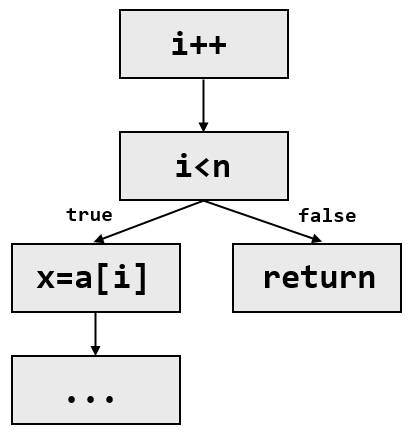
\includegraphics[width=0.3\textwidth]{images/symbolic_execution.png}
		\caption{Ausführungspfade für die symbolische Ausführung einer if-Anweisung}
\end{SCfigure}

Der aktuelle Zustand der Ausführung wird dabei durch zwei verschiedene Strukturen charakterisiert: 
Den Heap, der alle Elemente (engl. heap chunks) des Speichers beinhaltet sowie eine Liste
der geschlussfolgerten Annahmen (engl. assumptions). Bei der Ausführung der Vorbedingungen werden
diese Aussagen nun untersucht und entweder zum Heap hinzugefügt oder zu den Annahmen.

Beim Verstehen dieser Schritte ist die Verifast-Oberfläche sehr hilfreich, da sie den aktuellen
Zustand für einen beliebigen Haltepunkt anzeigen kann. Die folgende Situation zeigt die Ausführung
einer \lstinline{mismatch}-Implementierung bis zum gesetzten Haltepunkt (gelb hervorgehoben).

\begin{center}
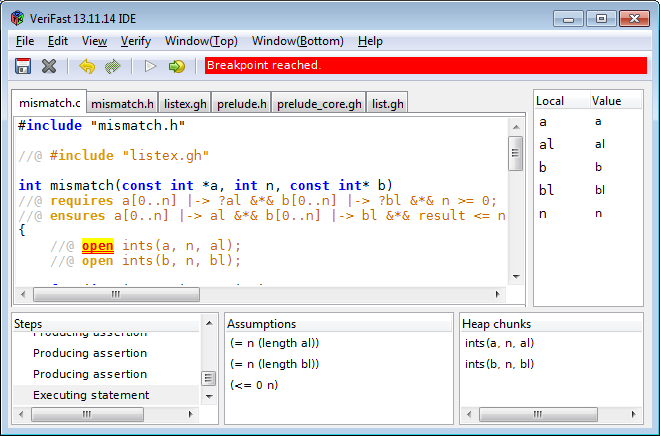
\includegraphics[width=1.0\textwidth]{images/verifast-state-after-precondition.png}
\end{center}

Gut zu erkennen ist, dass logische Ausdrücke wie \(n >= 0\) in die Liste der Annahmen 
(im Bild als \glqq Assumptions\grqq betitelt) aufgenommen wurden. Die \lstinline{ints}-Prädikate hingegen
wurden zum Heap hinzugefügt. Diesen Prozess nennt Verifast \glqq Producing assertion\grqq, wobei sich das Verb
\glqq Producing\grqq auf das Hinzufügen von Elementen zum aktuellen Zustand der symbolischen Ausführung
bezieht.

Das Gegenteil - \glqq Consuming assertion\grqq - findet z.B. beim Verifizieren der Nachbedingungen statt.
Verifast versucht dann alle erforderlichen Aussagen in der Liste der Annahmen bzw. im Heap zu finden
und diese, wenn sie denn passen, zu entfernen. Zusätzlich dazu wird am Ende einer Funktion - beim 
\glqq Leak check\grqq - auch überprüft, dass der Heap (der aktuellen Funktion) leer ist. Ist das nicht 
der Fall so wurde der entsprechende Speicher nicht korrekt bereinigt oder zumindest war Verifast nicht 
in der Lage das Gegenteil zu beweisen.

In dem Fall von mismatch würde Verifast die Heap chunks \lstinline{ints(a, n, al)} sowie
\lstinline{ints(b, n, bl)} beim Konsumieren der Nachbedingung auf dem Heap finden, entfernen und
somit erfolgreich verifizieren können, dass der Speicher so wie vor dem Aufruf vorhanden ist.



\section{Assertions und Ghost-Commands}

Zusicherungen (engl. assertions) und Ghost-Commands sind Annotationen, die direkt in den Implementierungs-Code
geschrieben werden. Assertions stellen sicher, dass der enthaltene Ausdruck wahr ist und sind ein nützliches Hilfsmittel, 
um die Verifizierung besser nachzuvollziehen als auch verständlicher zu machen. Insbesondere dann, wenn das Verifikationswerkzeug 
nicht triviale Schlüsse zieht, ist es von Vorteil Assertions zu ergänzen und im Code zu belassen.

Ghost-Commands hingegen enthalten Anweisungen für die Verifizierung, z.B. das Aufrufen anderer Sprachkonstrukte 
(z.B. Lemmata oder Fixpointfunktionen, siehe \ref{verifizierung:lemma}). Sie helfen dem Werkzeug logische Schlüsse 
zu ziehen, die es alleine nicht tun kann.
\newline
\newline
Der folgende Quellcode zeigt einen Ausschnitt aus einer rekursiven Implementierung für \lstinline{equal} und dient
hier als Anschauungsmaterial für die Erklärung der oben genannten Annotationstypen:

\lstinputlisting[language=C, caption=Rekursive Implementierung für \lstinline{equal} mit Verifast]{codes/equal_recursive_verifast.c}

Diese Implementierung zeigt nur die Abbruchbedingung der Rekursion - ist \lstinline{n == 0}, so sind die
leeren Listen gleich und die Berechnung terminiert. 

Die Zeilen 9 und 10 sind Assertions, die formal beschreiben, dass die induktiven Listen \lstinline{al} und
\lstinline{bl} die Länge 0 haben müssen und somit gleich lang sind. Damit Verifast in der Lage ist das zu
beweisen sind die zwei Ghost-Commands in Zeile 5 und 6 notwendig. Sie öffnen das \lstinline{ints}-Prädikat
und bringen somit dessen Inhalt in die Liste der Annahmen. Erst dadurch ist für Verifast ersichtlich, dass 
\lstinline{n} gleichzusetzen ist mit \texttt{length(al)} und \texttt{length(bl)}. Außerdem produziert
das Öffnen des Prädikats die Formel \lstinline{al = nil} bzw. \lstinline{bl = nil} (siehe Definition
des Prädikats in Listing 3.9 oder 4.2). Damit löst sich die Assertion \lstinline{al == bl} in den
trivialen Vergleich \lstinline{nil == nil} auf.
\newline
\newline
Das Öffnen der Prädikate konsumiert gleichzeitig auch die entsprechenden Heap-Chunks, was jedoch dazu führt,
dass diese beim Produzieren der Nachbedingung fehlen. Sie müssen also vor der \(return\)-Anweisung
wieder geschlossen werden (Zeile 11 und 12), damit sie dann wieder an den Aufrufer zurückgegeben werden können 
- so wie es die Nachbedingung verlangt.

Das Schreiben dieser \(close\)-Annotation ist jedoch oft nicht notwendig, da Verifast sie automatisch
einführt, wenn es sich um ein sogenanntes präzises Prädikat handelt. Darunter versteht Verifast Prädikate mit 
eingehenden und ausgehenden Parametern, die exakt die gleiche Speicherregion repräsentieren. 

\begin{figure}[H]
Die Kennzeichnung als präzises Prädikat geschieht über die Nutzung eines Semikolons bei der Trennung
der Prädikaten-Parameter:

\lstinputlisting[language=C, caption=Präzises Prädikat \lstinline{ints}]{codes/ints_precise_predicate_verifast.c}
\end{figure}
Präzise Prädikate versucht Verifast während der Verifizierung automatisch zu öffnen und ggf. auch zu
schließen. Dadurch ist in der obigen Implementierung das Schreiben der \texttt{close}-Anweisungen
nicht zwingend notwendig.
\newline
\newline
Assertions in ACSL werden genauso notiert wie in Verifast. Ghost-Commands hingegen werden
mit dem Schlüsseltwort \lstinline{ghost} eingeleitet, sind aber generell nicht so oft wie in
Verifast notwendig. Das kommt daher, dass Frama-C aufwendigere Berechnungen durchführt, um
entsprechende logische Schlüsse zu ziehen. Das ist jedoch auch spürbar, wenn man die
Geschwindigkeit der Werkzeuge vergleicht.


\section{Schleifeninvarianten}

schleifeninvarianten in acsl

alle angefassten variablen müssen per assigns erlaubt werden

dann in verifast zeigen

ähnlich, alles muss in invariante defniiert sein, was man benutzen will

toolunterstützung frama-c zeigen und erklären

\section{Lemmata und Axiome}
\label{verifizierung:lemma}

intsinv zeigen mit length

fixpoint nochmal zeigen (take)

erwähnen dass verifast terminierung von fixpount und lemmas prüft

\lstinline{take_one_plus} lemma zeigen

ggf. screenshot hier erst zeigen

erklären wieso es notwendig ist

\section{Speicherprobleme aufdecken}

malloc/free - chunks

zeigen an hand von main-funktion (unit-test)

verifast hilft klar zu dokumentieren wer für speicher verantwortlich ist (rufer oder gerufener)

\section{Überläufe erkennen}

overflow checken

\chapter{Vergleich weiterer Aspekte}


\section{Aliasing}

copy oder move zeigen und unterschied zwischen acsl und verifast

\lstinline{\seperated}


\chapter{Fazit}

Abschließend lässt sich sagen, dass beide Werkzeuge sehr gut geeignet sind, um die funktionalen Eigenschaften von
Algorithmen nachzuweisen. Für die einfachen Beispiele in dieser Arbeit ist Frama-C jedoch etwas passender, da die
entsprechenden Kontrakte einfacher zu schreiben sowie zu lesen sind.

VeriFast spielt seine Stärken bei komplizierten Datenstrukturen aus und dann wenn es neben den funktionalen Eigenschaften
auch oder ausschließlich um die Robustheit des Codes geht. Aktuell ist von den beiden Werkzeugen nur VeriFast in der Lage
eine korrekte Speicherverwaltung nachzuweisen.

Die beiden Werkzeuge verfolgen einen unterschiedlichen Ansatz. VeriFast hat eine intuitive Oberfläche, welche die Verifizierung
erleichtert - erwartet aber mehr Annotationen im Quellcode. Das liegt daran, dass der Beweiser bei der Arbeit mit Listen
nicht so mächtig ist wie die Frama-C-Beweiser beim Schlussfolgern im Zusammenspiel mit Quantoren aus der Prädikatenlogik.
Die mit VeriFast geschriebenen Kontrakte ähneln wegen der Nutzung von Listen und den dazugehörigen Fixpunktfunktionen
oft Programmen aus einer funktionalen Sprache wie Haskell. Personen mit einem solchen Hintergrund finden darum einen leichten Zugang zu
VeriFast. Wer aber bereits die Prädikatenlogik kennt oder auch interaktive Beweiser wie Coq, wird sich mit
dem WP-Plugin von Frama-C besser zurecht finden.


\begin{thebibliography}{}
\bibitem[jac12]{jacobs-tutorial} Bart Jacobs, Jan Smans, Frank Piessens: The VeriFast Program Verifier: A Tutorial, Dezember 2012
\bibitem[jac08]{jacobs-2008} Bart Jacobs, Frank Piessens: The Verifast Program Verifier, 2008
\bibitem[jac10]{jacobs-2010} Bart Jacobs, Jans Smans, Frank Piessens: Verifast: Imperative Programs as Proofs, 2010
\bibitem[jac10-1]{jacobs-2010-1} Bart Jacobs, Jan Smans, Frank Piessens: A Quick Tour of the VeriFast Program Verifier
\bibitem[rey02]{reynolds-2002} John C. Reynolds: Seperation Logic: A logic for shared mutable data structures, 2002
\bibitem[phi12]{casestudy} Pieter Philippaerts et al: Software Verification with VeriFast: Industrial Case Studies, 2012
\bibitem[hoare69]{hoare} C.A.R Hore: An axiomatic basis for computer programming, 1969
\bibitem[turing36]{turing} Alan Turing: On computable numbers, with an application to the Entscheidungsproblem, 1936
\bibitem[floyd67]{floyd} R. W. Floyd: Assigning meanings to programs, 1967
\bibitem[vafeiadis11]{concurrent} Viktor Vafeiadis: Concurrent seperation logic and operational semantics, 2011
\end{thebibliography}

\listoffigures

\end{document}

